\chapter{Ewaluacja i rezultaty}
\label{cha:ewaluacjaIRezultaty}
Poniższy rozdział zawiera opis testów przeprowadzonych w celu zbadania działania algorytmu animacji awatara. Przedstawiono w nim również otrzymane rezultaty i wnioski płynące z opracowanej walidacji.

% %---------------------------------------------------------------------------

\section{Sposób testowania}
Przetestowanie stworzonego programu to kluczowa kwestia, dzięki której łatwiej wykryć błędy mogące pojawić się podczas użytkowania danego oprogramowania. Istotna jest również opinia osób testujących program, niejednokrotnie zwracają oni uwagę na braki, których uzupełnienie potrafi zdecydowanie usprawnić korzystanie z aplikacji.

\begin{figure}[h]
	\centering
	\begin{subfigure}{0.35\textwidth}
		\centering
		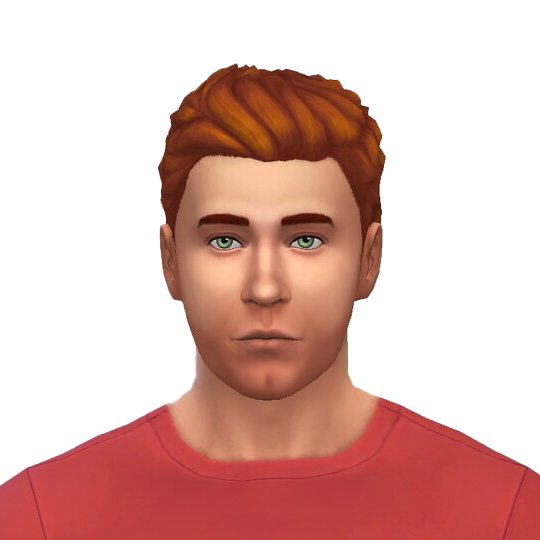
\includegraphics[height=4cm]{zdjęcia/1.png}
		\subcaption{\label{avatar_1}}
	\end{subfigure}
	\begin{subfigure}{0.35\textwidth}
		\centering
		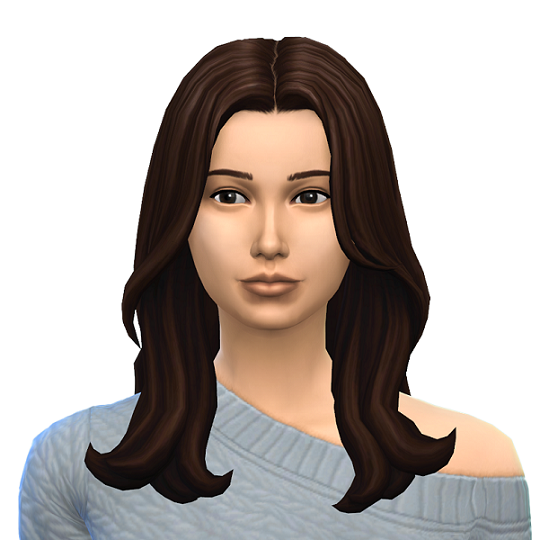
\includegraphics[height=4cm]{zdjęcia/2.png}
		\subcaption{\label{avatar_2}}
	\end{subfigure}
	\begin{subfigure}{0.35\textwidth}
		\centering
		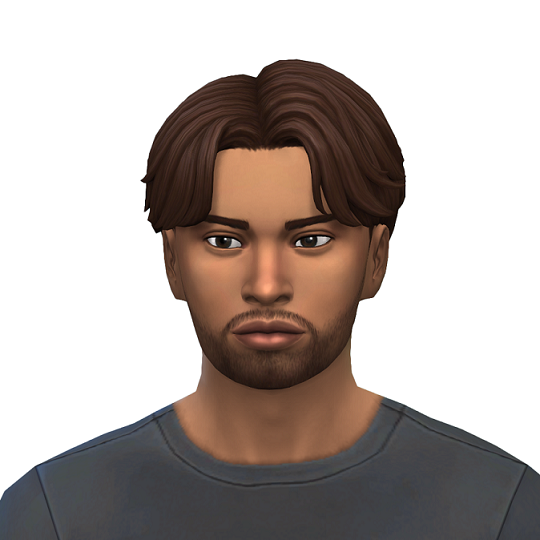
\includegraphics[height=4cm]{zdjęcia/3.png}
		\subcaption{\label{avatar_3}}
	\end{subfigure}
	\begin{subfigure}{0.35\textwidth}
		\centering
		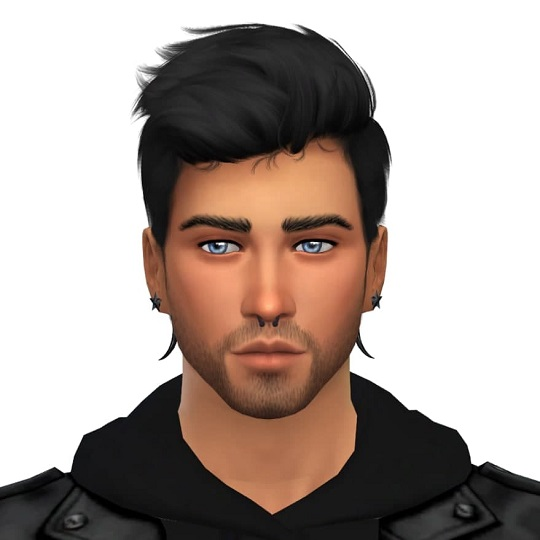
\includegraphics[height=4cm]{zdjęcia/4.png}
		\subcaption{\label{avatar_4}}
	\end{subfigure}
	
	\caption{\label{fig:avatars}Awatary użyte do przetestowania algorytmu}
\end{figure}

W czasie tworzenia algorytmu animacji awatara zostały przeprowadzone testy manualne poszczególnych funkcji, co pomogło usprawnić niektóre moduły i dopracować logikę ich działania. Ze względu na prostotę programu, stworzonego na potrzeby tej pracy inżynierkiej, wykonywanie bardziej zaawansowanych testów samego oprogramowania nie było konieczne.

Ważnym elementem stało się przetestowanie efektywności działania algorytmu na zarejestrowanych obrazach lub gotowych zbiorach danych, co wcześniej zostało określone w założeniach projektowych (sekcja \ref{sec:zalozeniaProjektu}). Z tego powodu przeprowadzono testy użyteczności, które zostały podzielone na dwie części. W każdej z nich modyfikowano zdjęcia czterech różnych awatarów \ref{fig:avatars}, co pozwoliło w lepszy sposób przetestować algorytm.

Dobór zdjęć do testowania algorytmu nie był przypadkowy. W ramach niniejszej pracy jako awatar rozumie się nierealną cyfrową postać mającą formę osobową. Ważną cechą jest prostota takiego charakteru - wyraźne rysy twarzy, brak cieni. Ze względu na owe wymagania do testów wybrano podobizny z popularnej gry symulacyjnej The Sims 4~\cite{avatars}, które zostały udostępnione na forum.

% %---------------------------------------------------------------------------

\section{Walidacja z użyciem aplikacji}
Pierwsza część przeprowadzonych testów obejmuje wykorzystanie aplikacji webowej w celu zbadania efektywności działania algorytmu w przypadku animacji na podstawie obrazu przechwyconego z kamery. 

Na potrzeby przeprowadzonego badania stworzono ankietę składającą się z czterech sekcji, gdzie każda dotyczy modyfikacji innego awatara. Głównym zadaniem ma być ocena rezultatów odwzorowania czterech podstawowych emocji \cite{emotions}, na które składają się:

\begin{itemize}
    \item szczęście,
    \item smutek,
    \item strach/zaskoczenie,
    \item gniew/obrzydzenie.
\end{itemize}

Każda sekcja złożona jest z pięciu pytań:
\begin{itemize}
    \item Cztery z nich dotyczą testowania zakładki \textit{Real-time animation}, gdzie awatar jest animowany na podstawie obrazu przechwyconego z kamery.
    \item Jedno ma na celu porówananie efektów otrzymanych przez animację opartą na analizowaniu obrazu z kamery z modyfikacją na podstawie wczytanego zdjęcia (zakładka \textit{Select image}).
\end{itemize}

Treść czterech pierwszych pytań różni się między sobą tylko emocją, którą aktualnie należy przetestować. Dla przykładu pierwsze pytanie ma postać:
\begin{center}
    Odwzorowanie pierwszej podstawowej emocji (szczęście).
\end{center}

W tej części zastosowano ocenianie za pomocą skali od 1 do 5, gdzie konkretnym wartościom odpowiadają następujące etykiety:
\begin{enumerate}
    \item Bardzo słaby
    \item Słaby
    \item Przeciętny
    \item Dobry
    \item Bardzo dobry

\end{enumerate}

\begin{table}[h]
\centering
\begin{tabular}{|c|l|c|c|c|c|c|} 
\hline
\multirow{2}{*}{\textbf{awatar}} & \multicolumn{1}{c|}{\multirow{2}{*}{\textbf{emocja}}} & \multicolumn{5}{c|}{\textbf{ocena}}                                                                                                   \\ 
\cline{3-7}
                                 & \multicolumn{1}{c|}{}                                 & \textbf{1} & \textbf{2} & \textbf{3}                       & \textbf{4}                         & \textbf{5}                          \\ 
\hhline{|=======|}
\multirow{4}{*}{\ref{avatar_1}}        & szczęście                                             & ~ 0\%~~    & ~ 9\%~~    & ~ 0\%~                           & \textcolor[rgb]{0,0.588,0}{~ 45\%} & \textcolor[rgb]{0,0.588,0}{~ 45\%}  \\ 
\cline{2-7}
                                 & smutek                                                & 0\%        & 0\%        & 0\%                              & \textcolor[rgb]{0,0.588,0}{64\%}   & 36\%                                \\ 
\cline{2-7}
                                 & zaskoczenie/strach                                    & 0\%        & 0\%        & 18\%                             & \textcolor[rgb]{0,0.588,0}{45\%}   & 36\%                                \\ 
\cline{2-7}
                                 & gniew/obrzydzenie                                     & 0\%        & 9\%        & 18\%                             & \textcolor[rgb]{0,0.588,0}{36\%}   & \textcolor[rgb]{0,0.588,0}{36\%}    \\ 
\hhline{|=======|}
\multirow{4}{*}{\ref{avatar_2}}           & szczęście                                             & 0\%        & 9\%        & 9\%                              & \textcolor[rgb]{0,0.588,0}{45\%}   & 36\%                                \\ 
\cline{2-7}
                                 & smutek                                                & 0\%        & 27\%       & 9\%                              & \textcolor[rgb]{0,0.588,0}{45\%}   & 18\%                                \\ 
\cline{2-7}
                                 & zaskoczenie/strach                                    & 9\%        & 0\%        & 27\%                             & \textcolor[rgb]{0,0.588,0}{55\%}   & 9\%                                 \\ 
\cline{2-7}
                                 & gniew/obrzydzenie                                     & 9\%        & 18\%       & \textcolor[rgb]{0,0.588,0}{45\%} & 27\%                               & 0\%                                 \\ 
\hhline{|=======|}
\multirow{4}{*}{\ref{avatar_3}}          & szczęście                                             & 0\%        & 0\%        & 9\%                              & \textcolor[rgb]{0,0.588,0}{45\%}   & \textcolor[rgb]{0,0.588,0}{45\%}    \\ 
\cline{2-7}
                                 & smutek                                                & 0\%        & 0\%        & 27\%                             & \textcolor[rgb]{0,0.588,0}{55\%}   & 18\%                                \\ 
\cline{2-7}
                                 & zaskoczenie/strach                                    & 0\%        & 9\%        & 18\%                             & \textcolor[rgb]{0,0.588,0}{36\%}   & \textcolor[rgb]{0,0.588,0}{36\%}    \\ 
\cline{2-7}
                                 & gniew/obrzydzenie                                     & 0\%        & 18\%       & 18\%                             & \textcolor[rgb]{0,0.588,0}{36\%}   & 27\%                                \\ 
\hhline{|=======|}
\multirow{4}{*}{\ref{avatar_4}}         & szczęście                                             & 0\%        & 0\%        & 0\%                              & 18\%                               & \textcolor[rgb]{0,0.588,0}{82\%}    \\ 
\cline{2-7}
                                 & smutek                                                & 0\%        & 9\%        & 0\%                              & \textcolor[rgb]{0,0.588,0}{55\%}   & 36\%                                \\ 
\cline{2-7}
                                 & zaskoczenie/strach                                    & 0\%        & 9\%        & 9\%                              & \textcolor[rgb]{0,0.588,0}{55\%}   & 27\%                                \\ 
\cline{2-7}
                                 & gniew/obrzydzenie                                     & 0\%        & 9\%        & 9\%                              & \textcolor[rgb]{0,0.588,0}{64\%}   & 18\%                                \\
\hline
\end{tabular}
\caption{Wyniki walidacji przeprowadzonej z użyciem aplikacji webowej}
\label{tab:first_test}
\end{table}

Ostatnie, piąte pytanie dotyczy oceny rezultatu osiągniętego w zakładce \textit{Select image} dla danego awatara. Osoba ankietowana powinna wybrać jedno zdjęcie z udostępnionej bazy odwzorowujące emocje, dla której rezultat animacji wypadł najgorzej. Następnie należy ocenić osiągnięty efekt, w stosunku do tego otrzymanego w zakładce \textit{Real-time animation}. Tym razem użyto skali od 1 do 7 gdzie 1 oznacza dużo gorszy efekt, natomiast 7 zdecydowanie lepszy wynik.

Przed przystąpieniem do testowania użytkownicy zostali zapoznani z krótką instrukcją, w której zwrócono uwagę na czynniki mogące mieć wpływ na działanie algorytmu:

\begin{enumerate}
    \item Ustaw twarz w pozycji frontowej, tak aby była ona dobrze widoczna w kamerze.
    \item Odsłoń włosy oraz zdejmij okulary.
    \item Staraj się nie wykonywać gwałtownych ruchów w momencie naciskania przycisku \textit{Animate}.
    \item W trakcie oceny rezultatów kieruj się głównie tym, czy emocja została poprawnie odwzorowana.
    \item Możesz wielokrotnie dokonywać animacji dla danej emocji i ocenić sumaryczne rezultaty.
\end{enumerate}

W ankiecie wzięło udział 11 osób w przedziale wiekowym od 19 do 60 lat. Większość z nich korzysta na co dzień z komputera, jednak tylko w podstawowych celach. W trakcie przeprowadzania ankiety nie wyniknęły żadne problemy. Aplikacja działała płynnie. Każdej osobie, bez żadnych przeszkód, udało się ukończyć zadania.

Procentowe wyniki ankiety przedstawiono w powyższej tabeli~(Tab.~\ref{tab:first_test}). Zawarto w niej efekty odpowiedzi na pytania 1-4, czyli te dotyczące odwzorowania danej emocji. Dla każdego awatara i dla wszystkich emocji dominujące wartości oznaczono kolorem zielonym. 

Analizując wyniki można dojść do następujących wniosków:
\begin{itemize}
    \item najlepsze oceny zanotowano dla awatara \ref{avatar_4}, odwzorowanie każdej z emocji zostało ocenione jako \textit{dobre} lub \textit{bardzo dobre} średnio w 89\% przypadków
    \item wyłącznie dla awatara \ref{avatar_2} i dwóch emocji odnotowano ocenę \textit{bardzo słaby}
    \item największą liczbę ocen \textit{bardzo słaby} oraz \textit{słaby} da się zauważyć dla awatara \ref{avatar_2} (średnio 18\% odpowiedzi)
\end{itemize}

Rozważając odpowiedzi na ostatnie pytanie, dotyczące porównania efektów osiągniętych w zakładce \textit{Select image} oraz \textit{Real-time animation}, można dojść do poniższych spostrzeżeń:
\begin{itemize}
    \item dla awatara \ref{avatar_1} w 91\% przypadków odpowiedzi skupiają się w przedziale od 4 do 7, co oznacza tendencję w kierunku oceny \textit{zdecydowanie lepszy}
    \item oceny awatara \ref{avatar_2} kumulują się między 1 a 4, zazwyczaj określając rezultaty jako \textit{gorsze}
    \item dla awatara \ref{avatar_3} koncentracja odpowiedzi przypada na przedział 4-7, aż w 45\% zdecydowano że efekt modyfikacji poprzez zakładkę \textit{Select image} jest \textit{zdecydowanie lepszy}
    \item efekty dla ostatniego awatara (\ref{avatar_4}) zostały ocenione bardzo różnorodnie, żadna z odpowiedzi nie wydaje się znacząco dominować
\end{itemize}


% %---------------------------------------------------------------------------

\section{Ocena osiągniętych efektów}
Druga część testów dotyczy oceny rezultatów osiągniętych poprzez zastosowanie algorytmu z wykorzystaniem gotowego zbioru danych. Celem tej części jest ocena wcześniej przygotowanych modyfikacji, co w przeciwieństwie do poprzedniej powinno dać przejrzyste wnioski. Wyniki poprzedniej części są obarczone błędem, ponieważ efekty mogą zależeć od mimiki poszczególnych osób biorących udział w badaniu. 

Przygotowanie danych przebiegało w następujący sposób:
\begin{itemize}
    \item wykorzystano bazę zdjęć zawierającą podobizny mężczyzn oraz kobiet z różnymi wyrazami twarzy, odpowiadającymi określonym emocjom
    \item dla każdej emocji, których podstawowy podział został podany w powyższym rozdziale, wybrano po jednym zdjęciu
    \item na podstawie wybranych obrazów dokonano modyfikacji każdego z awatara, finalnie otrzymano 16 przekształconych obrazów
\end{itemize}

\begin{table}[h]
\centering
\begin{tabular}{|c|c|c|c|c|} 
\hline
                                                              & \multicolumn{4}{c|}{awatar}                                                                                                                                                                \\ 
\hline
emocja                                                         & pierwszy                                   & ~ drugi~~                                 & ~ trzeci~~                                          & czwarty                                     \\ 
\hline
szczęście                                                      & ~ 74\%~~                                   & 70\%                                      & 85\%                                                & \textcolor[rgb]{0,0.502,0}{\textbf{100\%}}  \\ 
\hline
smutek                                                         & 78\%                                       & \textcolor[rgb]{0,0.502,0}{\textbf{93\%}} & 85\%                                                & 85\%                                        \\ 
\hline
zaskoczenie/strach                                             & \textcolor[rgb]{0,0.502,0}{\textbf{93\% }} & 74\%                                      & 63\%                                                & 63\%                                        \\ 
\hline
gniew/obrzydzenie                                              & 78\%                                       & 41\%                                      & \textcolor[rgb]{0,0.502,0}{\textbf{96\%}}           & 67\%                                        \\ 
\hline
\bottomrule
\begin{tabular}[c]{@{}c@{}}sumaryczna poprawność\end{tabular} & 81\%                                       & {\cellcolor{red}}\textcolor{white}{69\%}  & {\cellcolor[rgb]{0,0.502,0}}\textcolor{white}{82\%} & 79\%                                        \\
\hline
\end{tabular}
\caption{Ocena rezultatów osiągniętych z użyciem gotowego zbioru danych}
\label{tab:second_test}
\end{table}

Ankieta utworzona na potrzeby badania składa się z  16 pytań, każde z nich posiada cztery możliwe odpowiedzi:

\begin{enumerate}
    \item szczęście
    \item smutek
    \item strach/zaskoczenie
    \item gniew/obrzydzenie
\end{enumerate}



Zadaniem osoby ankietowanej była próba dopasowania emocji, którą odzwierciedla zmodyfikowany wyraz twarzy awatara. W celu łatwiejszego uporządkowania wyników zastosowano punktację 0-1. W ankiecie wzięło udział 27 osób w różnym przedziale wiekowym. Poniżej przedstawiono wartości najważniejszych parametrów otrzymanych wyników:
\begin{itemize}
    \item maksymalnie można było uzyskać 16 punktów
    \item najniższy uzyskany wynik to 9 punktów
    \item średni wynik to 12,44/16 punktów
    \item mediana wyniosła 12 punktów
\end{itemize}

\begin{figure}[h]
	\centering
	\begin{subfigure}{0.35\textwidth}
		\centering
		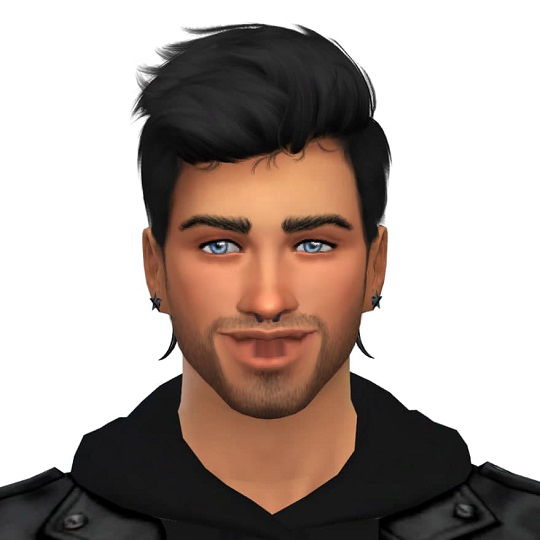
\includegraphics[height=4.5cm]{zdjęcia/av-4_happiness_2.png}
		\subcaption{\label{av-4_happiness_2}}
	\end{subfigure}
	\begin{subfigure}{0.35\textwidth}
		\centering
		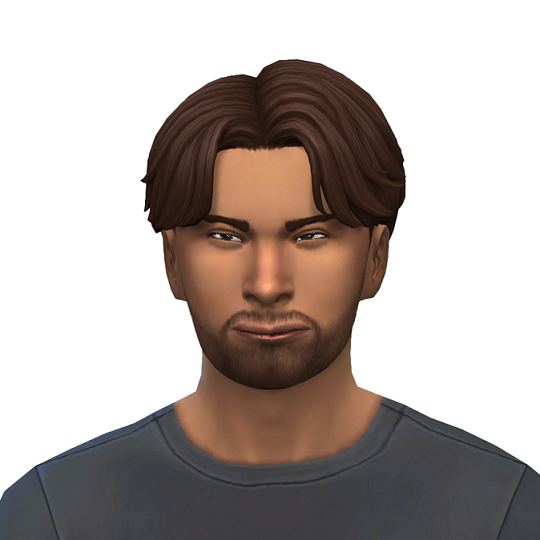
\includegraphics[height=4.5cm]{zdjęcia/av-3_anger_2.png}
		\subcaption{\label{av-3_anger_2}}
	\end{subfigure}

	
	\caption{\label{fig:best_results}Najtrafniej odgadnięte odwzorowania}
\end{figure}

Wyniki procentowe otrzymane po przeprowadzeniu badania zawarto w tabeli \ref{tab:second_test}. Po szczegółowej analizie, można zauważyć, że:
\begin{itemize}
    \item najwyżej oceniono awatar \ref{avatar_3} (82\% poprawnych odpowiedzi), a najgorzej \ref{avatar_2} (poprawność na poziomie 69\% )
    \item w odwzorowaniu szczęścia najwyższy wynik, bo aż 100\% otrzymano dla awatara \ref{avatar_4}
    \item wyraz twarzy dla smutku najtrafniej przyporządkowywano dla awatara \ref{avatar_2} (93\%)
    \item dla zaskoczenia/strachu największą poprawność dopasowania otrzymano dla awatara \ref{avatar_1} (93\%)
    \item najlepszy rezultat dla gniewu/obrzydzenia osiągnięto na awatarze \ref{avatar_3} (96\%)
\end{itemize}

Obrazy, których odzwierciedlane emocje przyporządkowano z najlepszą skutecznością (kolejno 100\% oraz 96\%) przedstawiono na Rys. \ref{fig:best_results}. Według ankietowanych obraz \ref{av-4_happiness_2} bardzo dobrze oddaje szczęście, mimo pewnego defektu w postaci braku uzębienia. Natomiast zdjęcie \ref{av-3_anger_2} poprawnie ukazuje gniew/obrzydzenie poprzez odpowiednie ułożenie ust oraz oczu. 

% %---------------------------------------------------------------------------

\section{Wnioski}
Przeprowadzone testy pomogły sprawdzić poprawność algorytmu zaimplementowanego w niniejszej pracy dyplomowej. Według użytkowników algorytm zapewnia dobre efekty, a stworzona aplikacja jest przyjemna i intuicyjna w użyciu. Wiele osób stwierdziło iż udział w badaniu był przyjemny i zapewnił odrobinę rozrywki.

Badania opisane w powyższym rozdziale pozwoliły na wykrycie wad oraz zdefiniowanie potencjalnych kierunków rozwoju i usprawnienia algorytmu. Kilku użytkowników zwróciło uwagę na brak uzębienia animowanych awatarów, który rozpraszał w trakcie testowania programu. Pojedyncza osoba wspomniała także o braku uwzględniania ułożenia brwi, co zdecydowanie udoskonaliłoby odczyt odwzorowania emocji.

Głównym celem było zbadanie jakości działania programu względem doboru awatara. Okazało się, że efektywność algorytmu w dużym stopniu zależy od obrazu, na którym następuje animacja. W pierwszej części testów najwyżej oceniono obraz \ref{avatar_4}, a w drugiej \ref{avatar_3}. Natomiast w obu najniżej oceniono awatar \ref{avatar_2}, na którym podczas modyfikacji pojawiało się sporo artefaktów psujących efekt animacji. Co więcej, ułożenie włosów kobiety znajdującej się na obrazie negatywnie wpływało na rezultaty, twarz nie zawsze układała się naturalnie. 

Istotną kwestią była także część, w której porównywano działanie algorytmu na gotowych obrazach z animacją \textit{real-time}. Dla awatarów ocenionych najwyżej efekty z obydwu zakładek były porównywalne, jednak dla gorszego awatara efektywność animacji na podstawie gotowych obrazów wzrastała. Może to być spowodowane Faktem jest, że rezultaty są mocno zależne od mimiki danej osoby, dla każdej z nich inny awatar sprawdzał się lepiej. 

Uważam, iż przeprowadzone testy przebiegły pomyślnie. Stworzona aplikacja okazała się dobrym narzędziem walidacji. Ewaluacja na gotowym zbiorze danych pomogła potwierdzić otrzymane wyniki oraz zwrócić uwagę na dodatkowe ścieżki rozwoju.



